% !TeX root = ../main.tex

\section{Bewegung}
\label{sec:movement}

\subsection{Iteration 1: Vorwärts und 90°-Drehung}
\label{sec:move-straight-turn}

Die erste Iteration diente der grundlegenden Bewegung des Dezibots auf dem Schachfeld. Also dem geradeaus Laufen und dem Rotieren um 90°. Hierzu wurde zunächst mit den bereits in der Dezibot-Library liegenden Funktionen experimentiert und aus den Erkenntnissen daraus hauptsächlich eigene Funktionen in der \texttt{ECPMovement}"=Klasse erstellt. 

\subsubsection{Farberkennung}
\label{sec:color-detection}

Damit der Dezibot sich eine bestimmte Anzahl an Feldern nach vorne bewegen kann, muss auf dem Schachbrett die Felder erkannt werden. Dies wurde mithilfe des RGBW"-Farbsensors auf der Unterseite des Dezibots angegangen. Dabei handelt es sich um einen \texttt{VEML6040}"=Farbsensor.

Die Experimente mit den Funktion \texttt{Color"-Detection::""get"-Color"-Value} führten zu unsinnigen Werten. Die meisten RGBW-Werte waren identisch, auch als der Dezibot auf rotem, blauen, grünem oder weißem Untergrund stand. Bei anschließender Recherche wurde die \texttt{VEML6040}"=Library~\footnote{\url{https://github.com/thewknd/VEML6040}} entdeckt. Diese liefert nachvollziehbare Werte. Dies führte zu der Entscheidung die \texttt{dezibot.color"-Detection}"=Klasse durch die neu implementierte Klasse \texttt{dezibot.color"-Sensor} zu ersetzen. Diese Änderung wurde auch in durch die Pull"-Request \texttt{Fix color detection library.}~\footnote{\url{https://github.com/dezibot/dezibot/pull/2}} in das Dezibot"=Repository gemerged, damit die anderen Gruppen ebenfalls eine funktionierende Farberkennung nutzen können.

Relevant für die Erkennung eines Feldes ist die Unterscheidung zwischen einem weißen (hellen) und einem schwarzen (dunklen) Untergrund. Dafür ist es notwendig die erhaltenen Farbwerte auf einer einheitlichen Skala zu normalisieren. In der Klasse \texttt{ECP"-Color"-Detection} wurden zudem die Methoden \texttt{is"-White"-Field} und später ein \texttt{turn"-On"-Color"-Correction"-Light} hinzugefügt, welche die notwendigen Operationen zusammenfassen. Probleme bestanden weiterhin durch die Abhängigkeit von dem Umgebungslicht. Die Idee bestand dadurch das normalisierte Umgebungslicht mit bei der Normalisierung zu berücksichtigen was zu der folgenden Formel zur Bestimmung eines Farbwertes, wobei $N_{C}$ der normalisierte Farbwert, $N_{A}$ das normalisierte Umgebungslicht, $M_{\texttt{RGBW}}$ der maximale Wert, der von dem Farbsensor wahrgenommen werden kann, und $M_{NC}$ der Maximale Farbwert nach der normalisierten Skala sind.

\begin{equation*}
    \begin{aligned}
        N_{C} = \min\{C \cdot \frac{N_{A}}{M_{\texttt{RGBW}}} \cdot M_{NC}, M_{NC}\}
    \end{aligned}
\end{equation*}

Für zuverlässigere Farbmessungen gerade bei schwachen Lichtverhältnissen wurde der Idee nachgegangen die LED auf der Unterseite des Dezibots anzuschalten um so möglichst gleichbleibendes Umgebungslicht bereitzustellen. Dies brachte deutliche Verbesserungen bei den Experimenten.

Für die Unterscheidung zwischen hellem und dunklem Untergrund wurde die Helligkeit mit den normalisierten Farbwerten approximiert~\footnote{Algorithmus vorgeschlagen in \url{https://www.w3.org/TR/AERT/#color-contrast}}. Dazu wurde in der Methode \texttt{Color"-Sensor::""calculate"-Brightness} die Farbwerte jeweils mit einem Faktor verrechnet. Anhand der Helligkeit wurde mit einem festgelegtem Schwellwerts zwischen einem weißen und schwarzen Feld unterschieden. Zusammengefasst wurde die Operation in der Methode \texttt{ECP"-Color"-Detection::""is"-White"-Field} bei der \textt{false} zurückgegeben wurde wenn die Helligkeit unter dem Schwellwert liegt und \texttt{true} sonst. Die gekürzte, konkrete Implementierung ist in \autoref{code:is-white-field} dargestellt.

 gegeben.

\begin{listing}[h]
    \inputminted{cpp}{../assets/code/ECPColorDetection.cpp}
    \caption{Vereinfachter Code"=Ausschnitt zur \texttt{ECP"-Color"-Detection::""is"-White"-Field}"=Methode}
    \label{code:is-white-field}
\end{listing}

Diese Lösung erfordert weitere Anpassungen im laufe des Projekts, da zunächst der Schwellwert kalibriert werden muss. Außerdem liegt der Farbsensor nicht in der Mitte des Dezibots, weshalb der hellste gemessene Farbwert und der dunkelste erreicht werden, wenn der Sensor in der Mitte eines Feldes ist und nicht wenn der gesamte Dezibot auf dem Feld steht.


\subsubsection{Implementierung}


\subsubsection{Experimente}

\begin{figure}[h]
    \centering
    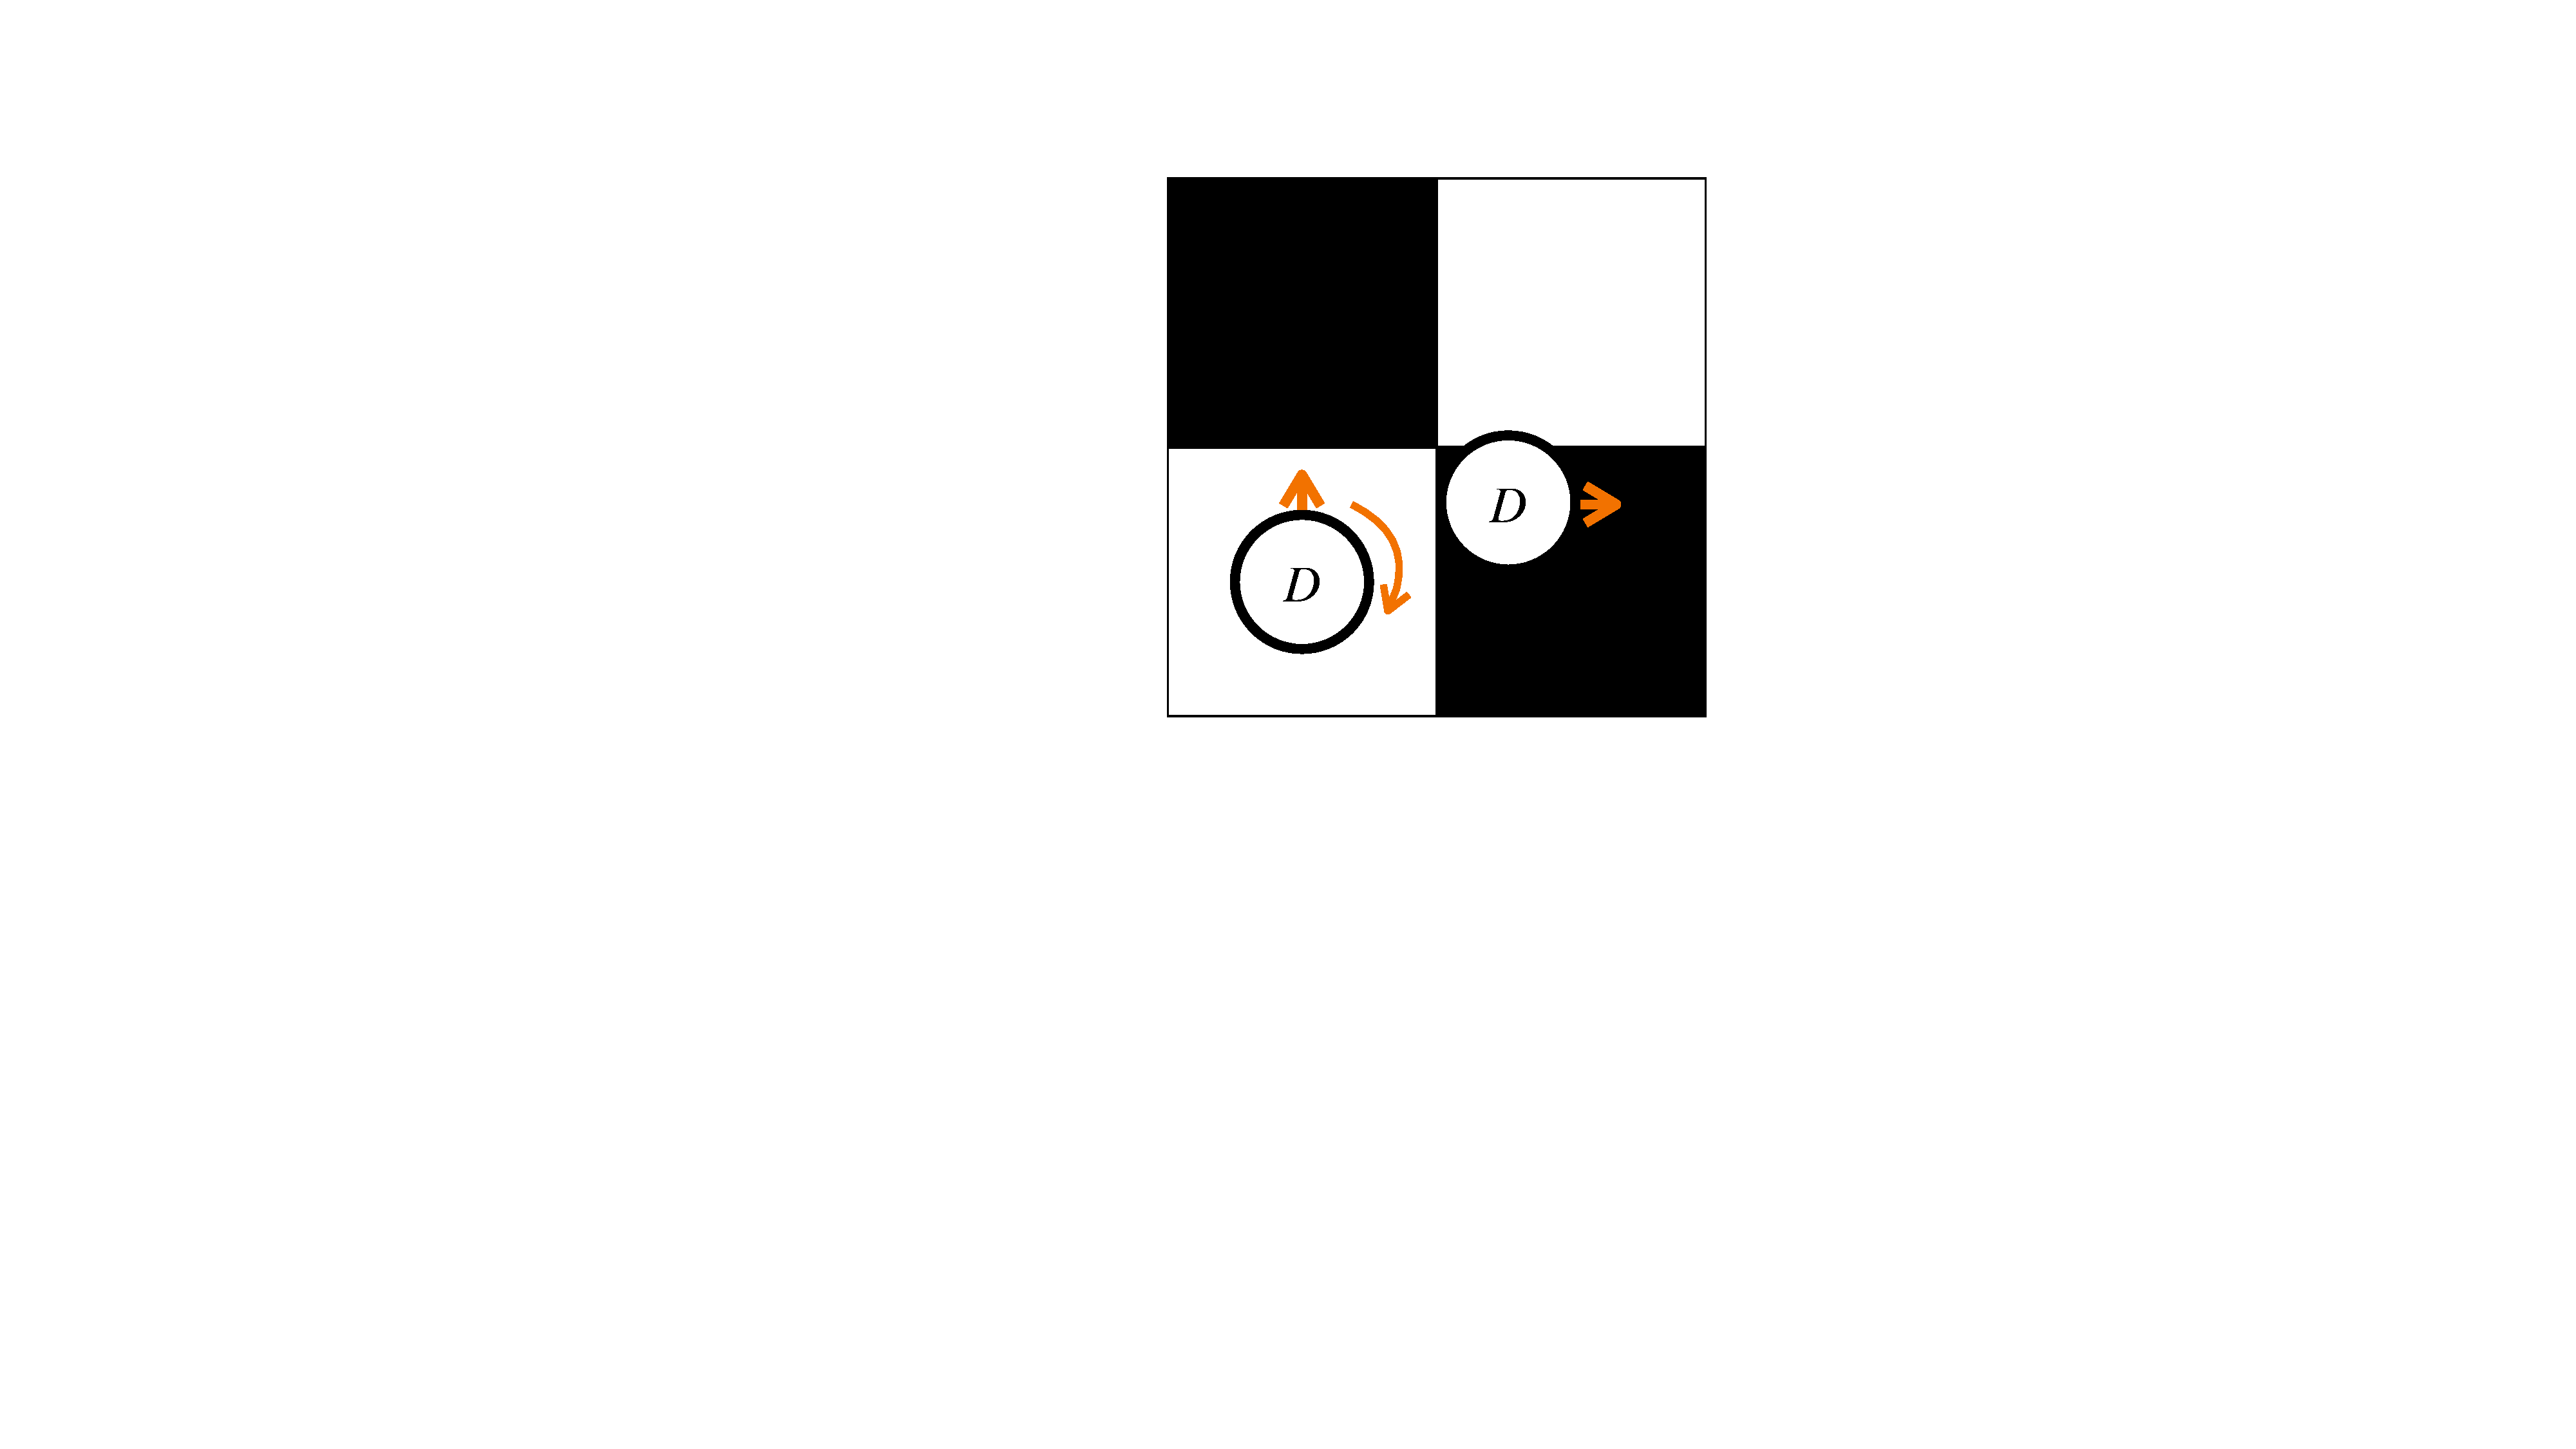
\includegraphics[width=0.4\textwidth]{../assets/dezibot_rotation_position_offset.pdf}
    \caption{90°"=Rechts"=Bewegung des Dezibots. Links ist Aus"-gangs-, rechts eine beispielhafte Endposition nach der Rotation abgebildet.}
    \label{fig:dezibot-rotation-position-offset}
\end{figure}


\subsection{Iteration 2: Allgemeine Move"=Funktion}
\label{sec:general-move-function}

Das Ziel der nächsten Iteration bestand darin, dem Dezibot nur ein Feld zu übergeben, auf das er sich bewegen soll. Somit entfällt die manuelle Berechnung, wie sich der Dezibot von seinem ursprünglichen auf ein gewünschtes Feld bewegt. Diese Funktion wurde in der \texttt{ECP"-Chess"-Piece::""move(ECP"-Chess"-Field new"-Field)}"=Funktion implementiert. Sie bewegt den Dezibot vom aktuellen Feld zum übergebenen \texttt{new"-Field}.

Dabei wird zunächst mit der \texttt{is"-Move"-Valid}"=Funktion überprüft, ob der gewünschte Zug gültig ist (vgl. \autoref{sec:move-validation}). Falls dem nicht so ist, werden die LEDs des Dezibots für eine bestimmte Zeit auf rot gestellt und \texttt{false} vorzeitig zurückgegeben. Hierbei wird der Dezibot also nicht bewegt. Andernfalls wird die Validität durch das Schalten der LEDs auf grün angezeigt und die notwendigen Bewegungen berechnet.

% Contraints: zurück rotieren

Dabei haben wir die folgenden Constraints aufgestellt: der Dezibot soll stets nach einem abgeschlossenen Zug in dieselbe Richtung schauen. Weiße Figuren schauen dabei stets in den Norden, schwarze in den Süden. Dies ist in orange in \autoref{fig:move-function-sketch} angedeutet.

\begin{figure}[h]
    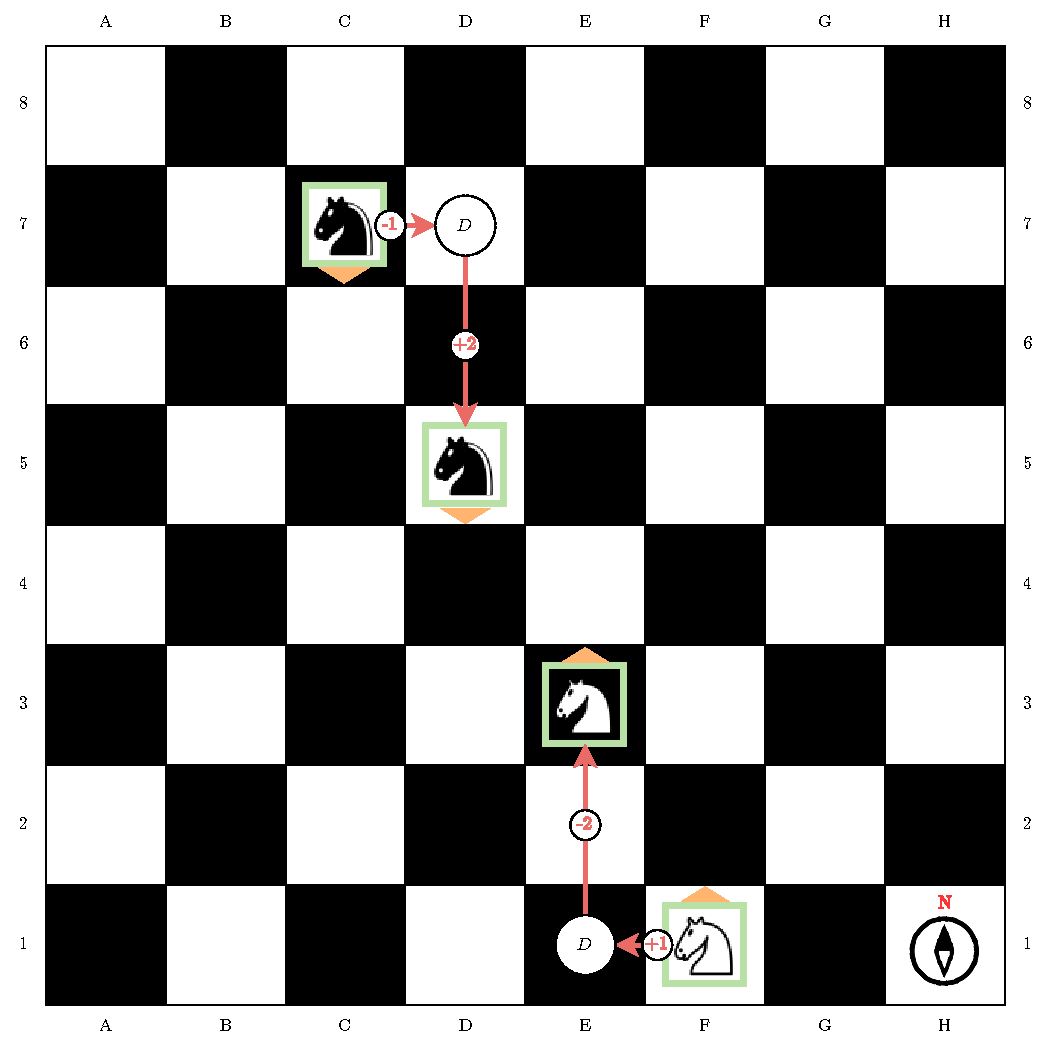
\includegraphics[width=\textwidth]{../assets/move_function_sketch.drawio.pdf}
    \caption{Veranschaulichung der Funktionalität von \texttt{move}. In orange ist die Ausrichtung des Dezibots, in rot die Differenz zwischen dem aktuellen und Zielfeld dargestellt.}
    \label{fig:move-function-sketch}
\end{figure}

% Zusammensetzung der Bewegung

Zunächst bewegt sich der Dezibot horizontal in die korrekte Spalte und anschließend vertikal in die richtige Zeile. Dafür wird die Spalten"= bzw. Zeilen"=Differenz vom aktuellen Feld zum neuen Feld berechnet.

\begin{equation*}
    \begin{aligned}
        \Delta\text{col} &= \text{col}_{\text{current}} - \text{col}_{\text{new}} \\
        \Delta\text{row} &= \text{row}_{\text{current}} - \text{row}_{\text{new}}
    \end{aligned}
\end{equation*}

Anschließend wird die horizontale Bewegung ausgeführt, falls $\Delta\text{col} \ne 0$ gilt. Entsprechend des Vorzeichens wird die neue Richtung bestimmt, d.h. ob der Dezibot sich nach Osten oder Westen drehen muss. Basierend auf der aktuellen Richtung des Dezibots, welche in \texttt{ECP"-Chess"-Pieces::""current"-Direction} gespeichert ist, wird berechnet, in welche Richtung sich der Dezibot rotieren muss. Anschließend bewegt sich der Dezibot um $\vert \Delta\text{col} \vert$ viele Felder vorwärts.

Ähnlich funktioniert die vertikale Bewegung. Die basiert auf der Zeilen"=Differenz $\Delta\text{row}$ sowie der Nord"=Süd"=Achse. Erneut wird berechnet, wie rotiert werden muss. Danach folgt die Vorwärtsbewegung um $\vert \Delta\text{row} \vert$ Felder.

Nachdem der Dezibot auf dem korrekten Feld steht, dreht sich der Dezibot zurück in die initiale Richtung. Somit drehen sich weiße Figuren wieder nach Norden; schwarze Figuren nach Süden. Somit ist die Bewegung zum gewünschten Feld abgeschlossen.

% Diskussion / Probleme

Insgesamt ergibt sich aus dem oben genannten Constraintsystem folgende Überlegungen. Es ergibt sich der Nachteil, dass sich die Rotationsfehler, auf welche in \autoref{sec:plausibility-check-rotation} genauer eingegangen wird, addieren. Allerdings ist das Display nach einem abgeschlossenen Zug stets gleich zur spielenden Person ausgerichtet. Dadurch sieht das Schachbrett optisch einheitlich aus, da alle Figuren derselben Farbe in dieselbe Richtung schauen, wodurch die Optik mehr einem echten Schachbrett entspricht. Weiterhin werden Display"=Ausgaben korrekt und nicht kopfüber dargestellt, wodurch diese einfacher durch die entsprechende spielende Person abzulesen sind. Ein weiterer Vorteil besteht in der darin, dass sich die Züge stets aus einer einheitlichen Bewegungs"- und Rotationsreihenfolge zusammensetzt, wodurch diese vorhersehbar ist. Somit überwiegen die Vorteile des Contraintsystems, besonders wenn das Probleme der Rotationsfehler behoben ist.


\subsection{Iteration 3: Plausibilitätsprüfung der Rotation}
\label{sec:plausibility-check-rotation}

Wie bereits in \autoref{sec:move-straight-turn} erwähnt, ist die Rotation nach einer fest definierten Zeit aufgrund von unvorhersehbaren äußeren Einflüssen unzuverlässig und führt meist nicht zum gewünschten Ergebnis. Weiterhin rotiert der Dezibot nicht auf einem \enquote{Fleck}, sondern bewegt sich an eine andere, nicht vorhersehbare Position. Dabei kann es passieren, dass der Dezibot, der ursprünglich auf einem weißen Feld stand, anschließend auf einem schwarzem steht (vgl. \autoref{fig:dezibot-rotation-position-offset}) oder vice versa. Daher wurde eine Plausibilitätsprüfung für die Rotation als Verbesserung eingeführt, welche überprüft, ob die Farbe des initialen Feldes dieselbe ist, wie die jenes Feldes, welches nach einer Rotation erreicht wurde.

Bei einer Rotation wird zunächst mit der in \autoref{sec:move-straight-turn} erwähnten \texttt{ECP"-Color"-Detection::""is"-White"-Field}"=Funktion gemessen, ob der Dezibot ursprünglich auf einem weißen oder schwarzem Feld steht. Nach einer Rotation wird dies erneut gemessen und mit dem ursprünglichen Wert verglichen. Wenn die Farben übereinstimmen, wird die Rotation als erfolgreich gewertet. Andernfalls wird eine Nachricht auf dem Display des Dezibots angezeigt, welche eine manuelle Korrektur anfordert. Dabei wird das gewünschte Feld sowie die Richtung, nach der der Dezibot ausgerichtet werden soll, ausgegeben. Eine Beispiel"=Ausgabe ist in \autoref{fig:display-rotation-correction-request} dargestellt.

\begin{figure}[h]
\centering
\begin{cminted}{text}
+----------------+
|Faulty rotation |
|Please correct  |
|my position in  |
|10 seconds to   |
|                |
|> A1 NORTH      |
|                |
|Thank you!      |
+----------------+
\end{cminted}
\caption{Beispiel für Aufforderung zur Korrektur einer fehlgeschlagenen Rotation. Gewünscht ist Feld \texttt{A1} mit Ausrichtung Norden.}
\label{fig:display-rotation-correction-request}
\end{figure}

Somit können fehlerhafte Rotationen, welche den Dezibot unerwünscht auf ein anderes Feld bewegen, von der nutzenden Person korrigiert werden. Dabei gilt jedoch die Einschränkung, dass der Dezibot auf ein Feld einer anderen Farbe rotieren muss, damit die Korrektur funktioniert. Falls bspw. von einem schwarzen auf ein anderes schwarzes Feld rotiert wird, kann dies mit diesem Ansatz nicht erkannt werden. Erfahrungsgemäß ist dies jedoch selten der Fall, da ein Dezibot sich sonst über zwei Felder (von schwarz zu weiß zu schwarz) bewegen müsste.

Mit dieser Verbesserung kann ebenfalls nicht überprüft werden, ob eine intendierte 90°"=Drehung den Dezibot auch tatsächlich um 90° dreht. Dieses Problem wurde in der folgenden Iteration thematisiert.


\subsection{Iteration 4: Infrarot"=basierte Rotation}
\label{sec:movement-ir}

Zur Verbesserung der Rotation wogen wir einige Ideen ab. Einerseits bauten wir bereits die im vorherigen Abschnitt erläuterte Plausibilitätsprüfung der Rotation ein. Eine zusätzliche Idee war es, ein Regelsystem für die Rotation zu entwerfen und zu implementieren. Dafür hatten wir verschiedene Ideen. Die Farbe bzw. das Licht vom Untergrund wird bereits die Plausibilitätsprüfung betrachtet. Insgesamt war der Wunsch, eine zweite physikalisch Größen einzubeziehen.

Der Beschleunigungssensor (\emph{Inertial Measurement Unit}, IMU) entfiel dabei als mögliche Option, da diese aktuell nur im Ansatz von der existierenden \texttt{dezibot}"=Library unterstützt wird und viel Low"=Level"=Code notwendig wäre. Außerdem hörten wir Berichte anderer Kommiliton:innen, welche eher negativ ausfielen.

Eine weitere Idee war es, Linien auf dem Schachbrett zu zeichnen und an andere Projekte anzuknüpfen, welche eine Linienverfolgung beinhalten. Dieser Ansatz wird im \autoref{sec:perspective} zum Ausblick noch einmal aufgegriffen. Da die entsprechenden Projekte damals allerdings noch nicht fertiggestellt waren und wir die Projekte nicht doppeln wollten, entschieden wir uns für den folgenden, anderen Ansatz.

Dieser Ansatz in einer zusätzlichen Signalquelle, welcher beispielsweise von einem weiteren Dezibot ausgesendet wird, und Trigonometrie. Vorstellbar sind hier WLAN- oder Bluetooth"=Signale, oder auch Infrarot"=Licht. Schlussendlich entschieden wir uns durch die Abwägung von Kosten und Nutzen für eine Infrarot"=LED als \emph{Beacon} sowie die seitlichen "=Sensoren zur Messung. Diese sind in \autoref{fig:dezibot-bottom} hervorgehoben.

\begin{figure}[h]
    \centering
    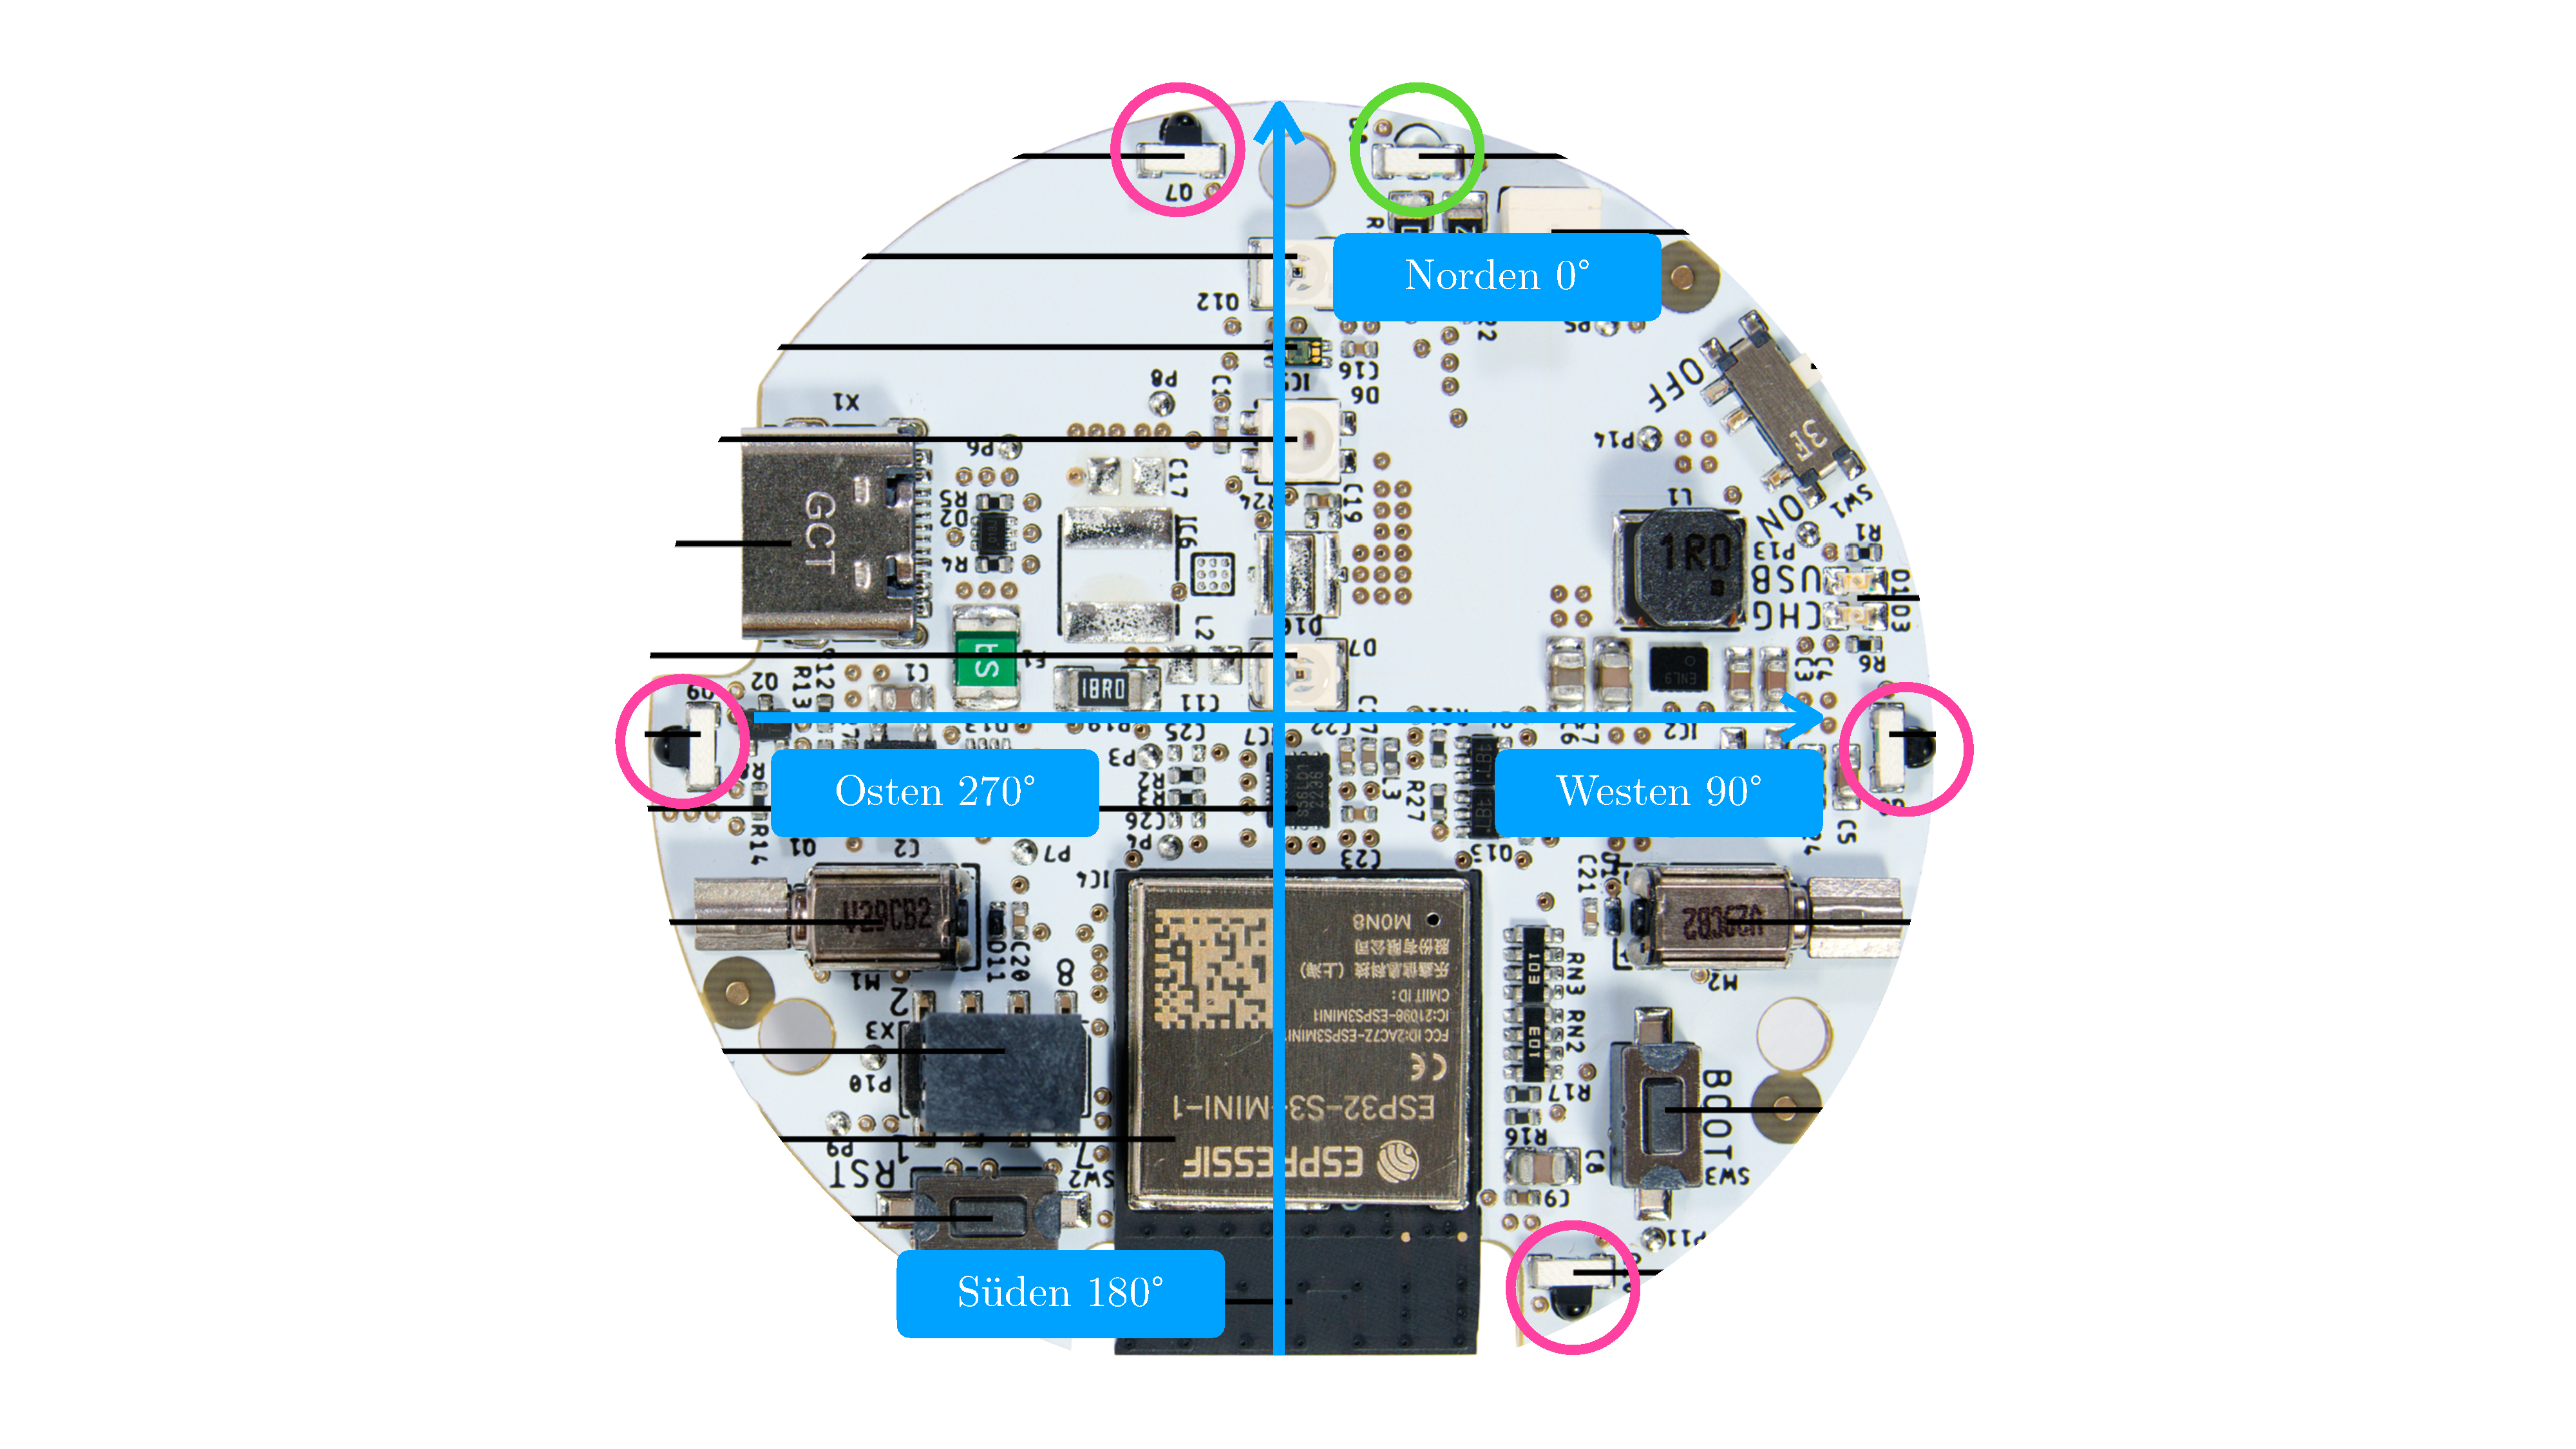
\includegraphics[width=0.8\textwidth]{../assets/dezibot_bottom.pdf}
    \caption{Unterseite des Dezibots, auf der die verwendete Infrarot"=LED in grün sowie die seitlichen Infrarot"=Sensoren in magenta umrandet sind. In blau sind die Himmelsrichtungen mit den entsprechenden (relativen) Winkel der Dezibot"=Ausrichtung eingezeichnet. West und Ost sind hier gespiegelt, da es sich hierbei um die Unterseite des Dezibots handelt. Grafik wurde aus~\cite{fingerleDokumentationDezibot42025} entnommen, bearbeitet und annotiert.}
    \label{fig:dezibot-bottom}
\end{figure}

Dafür wird ein Dezibot platziert, welcher ein Infrarot"=Signal aussendet, neben das Schachbrett platziert, welches ungefähr in die Mitte des Schachbretts schaut. Dafür wurde das Programm \href{https://github.com/nicosrm/24-emb-chess/blob/feature/31-rotation-infrared/example/EmbeddedChessPieces/examples/ir_sensors/ir_emitter/ir_emitter.ino}{\texttt{ir\_emitter.ino}} geschrieben, welches ebenjene Funktion erfüllt.

Dieses Signal wird von \texttt{ECP"-Signal"-Detection::""measure"-Signal"-Angle()} gemessen. Dabei werden der Werte von allen vier Infrarot"=Sensoren gelesen und verrechnet. Aus dem gemessenen Winkel des Beacon"=Signals wird der Winkel berechnet, in den der Dezibot in Relation zum Beacon ausgerichtet ist (vgl. \texttt{ECPSignal"-Detection::""measure"-Dezi"-bot"-Angle}). Die beiden Winkel sind in \autoref{fig:signal-dezibot-angle} verdeutlicht. Die Bestimmung der Winkel wird in \autoref{sec:angle-determination} genauer erläutert.

\begin{figure}[h]
    \centering
    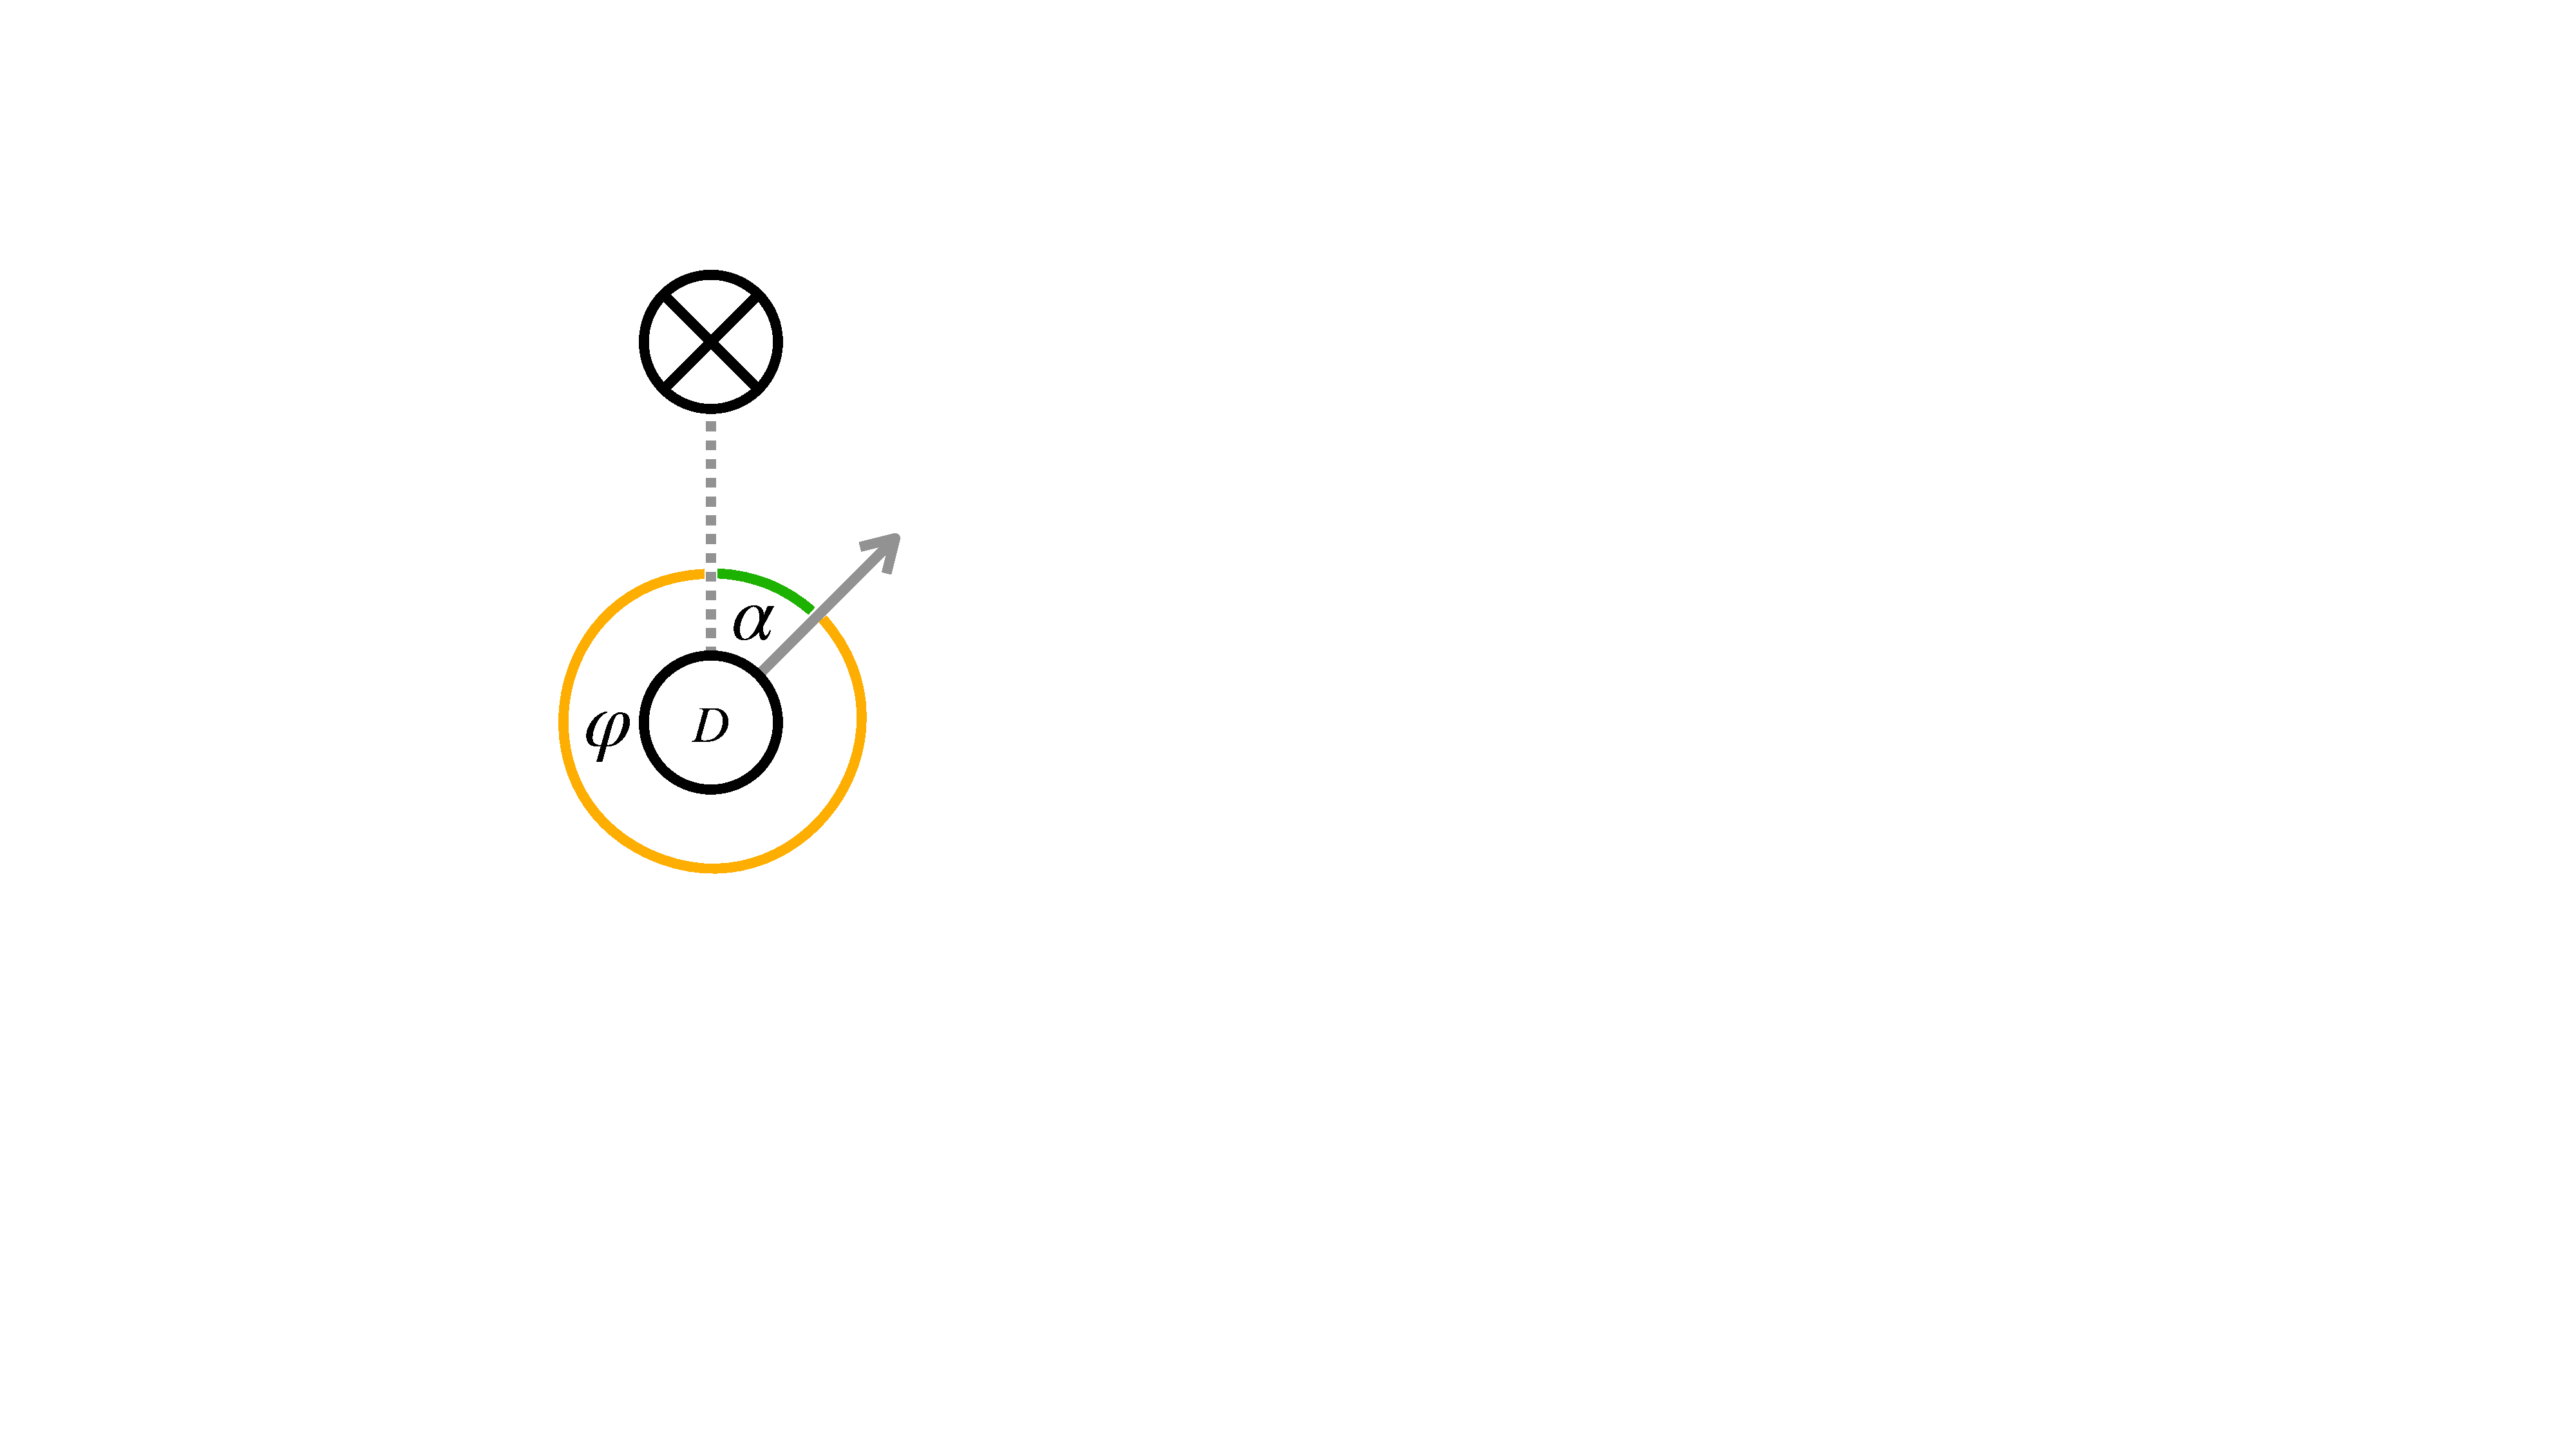
\includegraphics[width=0.2\textwidth]{../assets/signal_dezibot_angle.pdf}
    \caption{Skizze zur Darstellung des gemessenen Signal"=Winkels $\varphi$ vom Beacon sowie des dazu relativen Dezibot"=Aus"-rich"-tungs"-winkels~$\alpha$. $D$~markiert den messenden Dezibot, $\otimes$~den Beacon. Der von $D$ ausgehende graue Pfeil, zeigt die Ausrichtung des Dezibots an.}
    \label{fig:signal-dezibot-angle}
\end{figure}

Nachdem der Winkel berechnet wurde, wird ein Ziel"=Winkel~$\alpha'$ berechnet. Wenn sich der Dezibot nach links drehen soll, werden 90° vom initialen Winkel~$\alpha$ subtrahiert, bei einer Rotation nach rechts 90° addiert. Damit der Winkel bei einer Links"=Rotation nicht negativ wird, werden zunächst 360° addiert. Anschließend wird auf den Wert der Modulo 360 angewendet. Insgesamt folgt ein Ziel"=Winkel~$\alpha' \in [0,360] \subset \mathbb{N}$.

\begin{equation*}
\begin{aligned}
    \text{Rotation links } &\implies \alpha' = (\alpha - 90\degree + 360\degree) \operatorname{mod} 360\degree \\
    \text{Rotation rechts } &\implies \alpha' = (\alpha + 90\degree) \operatorname{mod} 360\degree
\end{aligned}
\end{equation*}

An diesem Punkt sind die zwei wichtigen Größen bekannt: einerseits der initiale Winkel~$\alpha$, in dem der Dezibot relativ zum Beacon \emph{vor} der Rotation steht; andererseits der relative Ziel"=Winkel~$\alpha'$, in dem der Dezibot nach der Rotation ausgerichtet sein soll. Eine Skizze ist in \autoref{fig:dezibot-rotation-angles} abgebildet.

\begin{figure}[h]
    \centering
    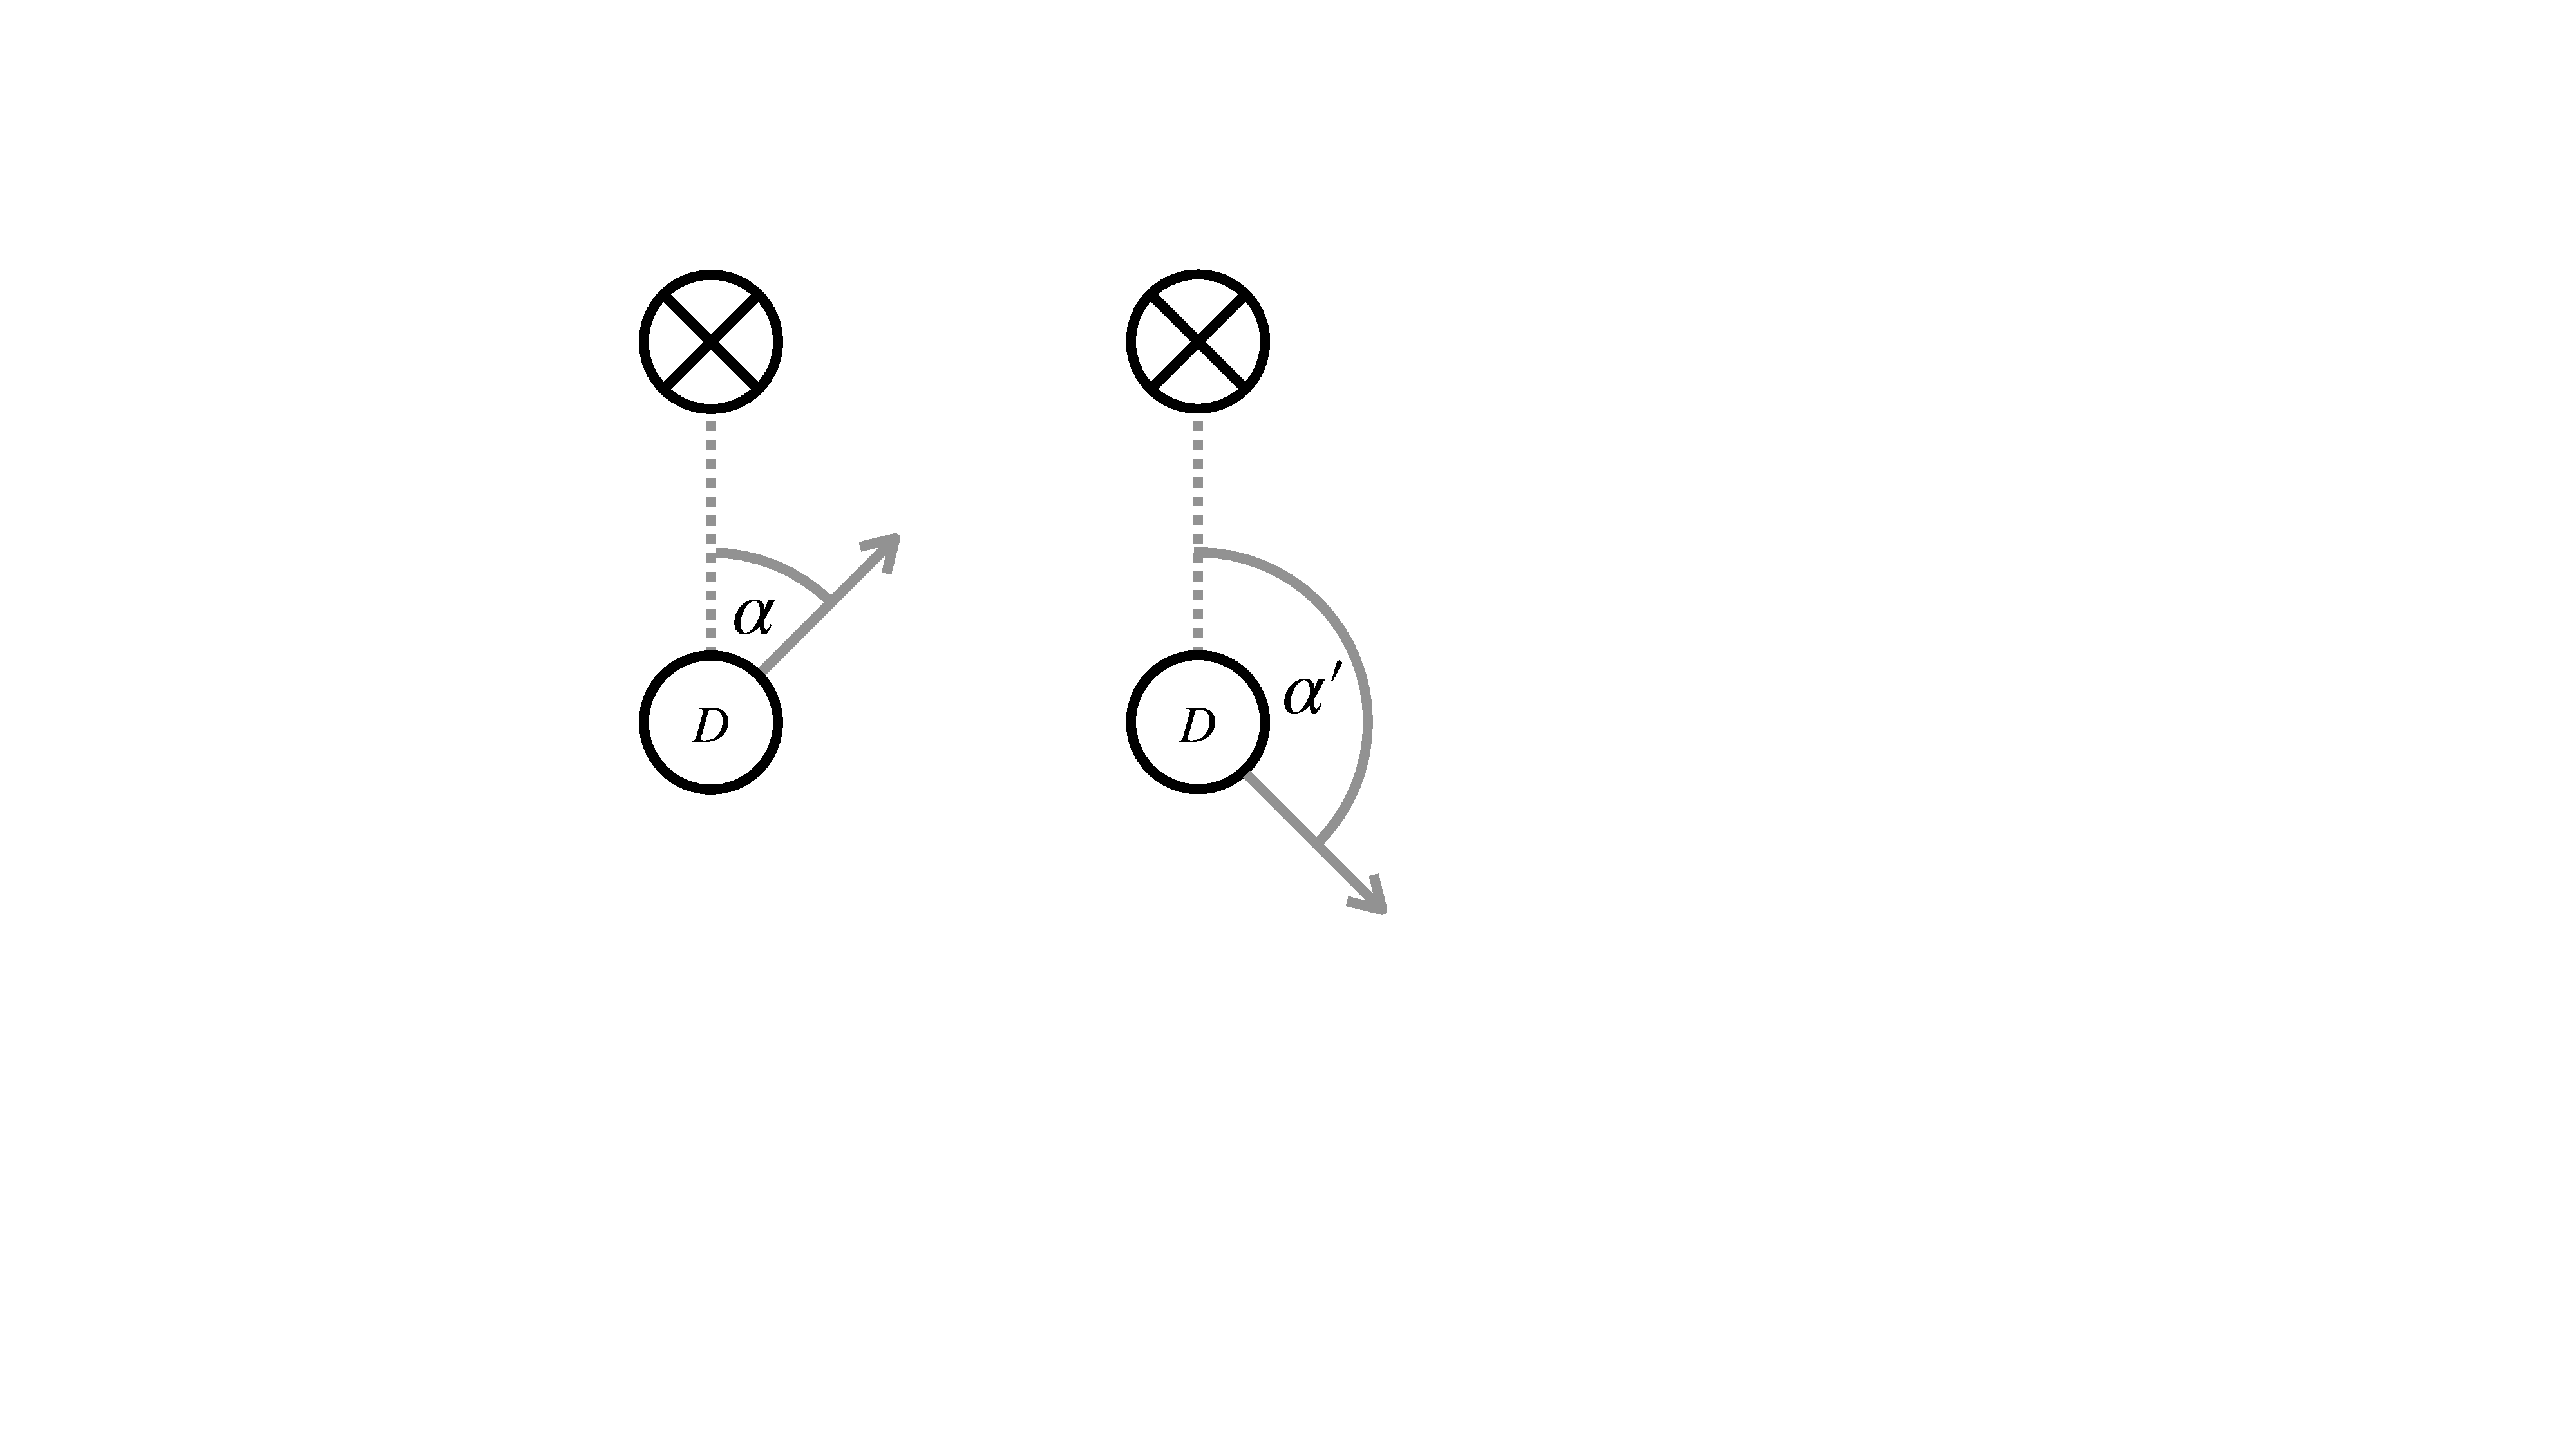
\includegraphics[width=0.5\textwidth]{../assets/dezibot_rotation_angles.pdf}
    \caption{Rotation des Dezibots vom initialen Winkel $\alpha$ (linke Seite) zum Ziel"=Winkel $\alpha'$ (rechte Seite). $D$~markiert den rotierenden Dezibot, $\otimes$~den Beacon. Der von $D$~ausgehende graue Pfeil, zeigt die Ausrichtung des Dezibots an.}
    \label{fig:dezibot-rotation-angles}
\end{figure}

Mit diesen beiden Werten wird die \texttt{ECPMove"-ment"-::"-rotate"-To"-Angle}"=Funktion aufgerufen. Diese rotiert den Dezibot inkrementell vom übergebenen initialen Winkel zum Ziel"=Winkel. Dabei wird innerhalb einer Schleife basierend auf der normalisierten Differenz $\Delta\theta_{\text{norm}}$ bestimmt, ob der Dezibot am effizientesten nach links oder rechts rotieren muss, um $\alpha'$ zu erreichen. Dies wird in \autoref{sec:rotation-direction-determination} genauer erläutert. Anschließend wird benötigte die Rotationszeit approximiert.

Die Approximation basiert auf empirischen Werten, welche ergeben haben, dass eine Rotation um 180° in etwa 5 Sekunden benötigen. Basierend auf der absoluten normalisiert Differenz $\vert\Delta\theta_{\text{norm}}\vert$ wird der folgende angenommene Approximation verwendet:

\begin{equation*}
    180\degree \cdot 28~\frac{\text{ms}}{\degree} = 5040~\text{ms} \approx 5000~\text{ms}
\end{equation*}

Dementsprechend ergibt sich die approximierte Rotationszeit $t_{\text{rot}}$ wie folgt:

\begin{equation*}
    t_{\text{rot}} \approx \vert\Delta\theta{\text{norm}}\vert \cdot 28~\frac{\text{ms}}{\degree}
\end{equation*}

Dementsprechend wird die approximierte Rotationszeit geringer, je kleiner die normalisierte Differenz wird. Das heißt, je näher sich der Dezibot am gewünschten Ziel"=Winkel $\alpha'$ ausgerichtet ist, desto kürzer wird rotiert.

Anschließend wird entsprechend der linke oder rechte Motor des Dezibots -- je nach kürzester bestimmter Rotationsrichtung -- für $t_{\text{rot}}$ aktiviert, wodurch der Dezibot in die jeweils entgegengesetzte Richtung rotiert.

Nach dem Rotationsinkrement wird der neue relative Winkel des Dezibots erneut gemessen, d.h. $\alpha$ aktualisiert, und die Iteration von vorn durchgeführt. Die Rotationsrichtung und "=zeit werden erneut berechnet, wodurch ein Gegensteuern möglich ist, falls sich der Dezibot zu weit bewegt hat. Eine Rotation wird außerdem als erfolgreich bewertet, wenn der neue Winkel $\alpha$ innerhalb einer festgelegten Toleranz -- aktuell 3° -- befindet. Diese Toleranz ist in \texttt{ECPMove"-ment::""ROTA"-TION\_TOLER"-ANCE} definiert.

Falls innerhalb von 20 Iterationen der Ziel"=Winkel nicht erreicht werden konnte, wird eine entsprechende Meldung auf das Display gedruckt. Diese fordert den Nutzenden auf, den Dezibot am entsprechenden Ziel"=Winkel auszurichten. Dies trat bei den Tests insignifikant wenig auf und ist als \emph{Fallback} gedacht.


\subsubsection{Bestimmung der Winkel}
\label{sec:angle-determination}

In diesem Abschnitt wird die Bestimmung des Winkels, in dem das Infrarot"=Signal beim Dezibot eintrifft, $\varphi$ sowie wie der Dezibot in Relation dazu ausgerichtet ist $\alpha$ bestimmt wird. Diese Funktionalitäten entsprechen den Funktionen \texttt{measure"-Signal"-Angle} sowie \texttt{measure"-Dezi"-bot"-Angle} aus \texttt{ECPSig"-nal"-Detec"-tion} Die Winkel sind in \autoref{fig:dezibot-rotation-angles} skizziert.

Zunächst werden die vier Werte der seitlichen Infrarot"=Sensoren gelesen. Dabei werden jeweils drei Messungen mit einem Abstand von jeweils einer Millisekunde gemittelt, um die Ergebnisse zu verbessern. Die Ergebnisse liegen auf einer Skala von $[0,4095]$ vor, welche zunächst auf $[0,1] \subset \mathbb{R}$ normalisiert wird, um eine leichtere Weiterverarbeitung zu ermöglichen. Anschließend wird überprüft, ob mindestens ein Messwert über einem festgelegten Schwellwert -- aktuell 0.1, d.h. 10 Prozent -- liegt, um eine gewisse Signalstärke vorauszusetzen. Falls dies nicht der Fall ist, wird eine entsprechende Warnung auf das Display gedruckt. Nach einer Sekunde wird erneut versucht, einen gültigen Wert zu lesen. Dies geschieht solange, bis ein signifikanter Wert gemessen werden kann.

Nachdem hinreichende Signalmessungen vorliegen, kann der Winkel Beacon"=Signals berechnet werden. Dazu werden die Nord"=Süd"? $r_{N,S}$ sowie Ost"=West"=Resultanten $R_{E,W}$ berechnet. Dabei sind $n,s,e$ und $w$ jeweils die Signalmessungen aus dem Infrarot"=Sensor aus Nord"=, Süd"=, West"= bzw. Ost"=Richtung.

\begin{equation*}
    r_{N,S} = n - s \qquad r_{E,W} = e - w
\end{equation*}

Aus diesen Resultanten wird der Winkel $\varphi$ vom Ergebnisvektor berechnet.

\begin{equation*}
    \varphi = \arctan_2(r_{E,W}, r_{N,S}) \cdot \frac{180\degree}{\pi}
\end{equation*}

Eine Veranschaulichung der Resultanten, des Ergebnisvektors sowie des Winkels~$\varphi$ sind anhand von Beispiel"=Daten in \autoref{fig:angle-determination-beacon} abgebildet.

\begin{figure}[h]
    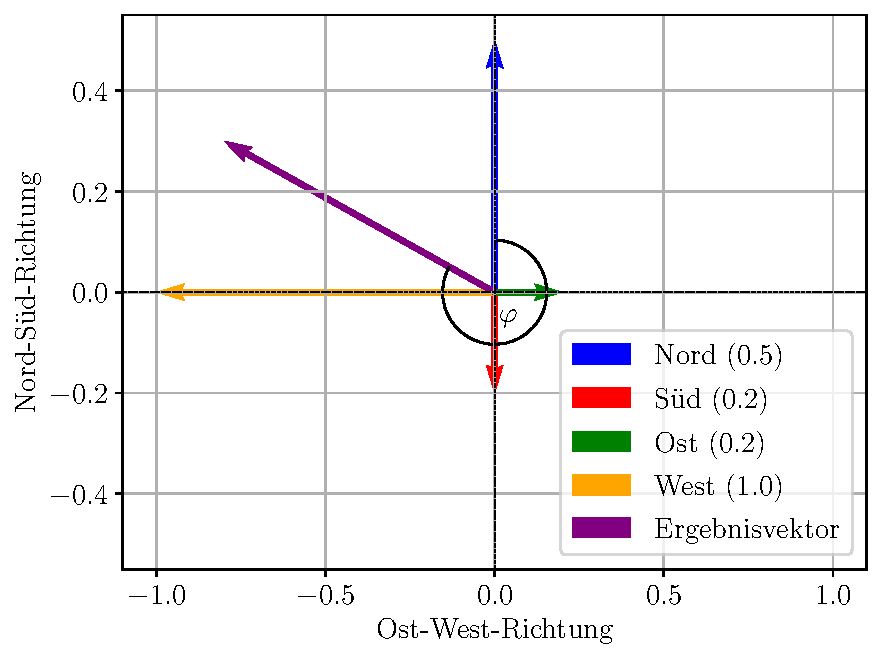
\includegraphics[width=\textwidth]{../plot/signal_direction.pdf}
    \caption{Veranschaulichung der Berechnung des Signal"=Winkels~$\varphi$ anhand eines Beispiels; Messwerte siehe Legende. Grafik wurde mittels \href{https://matplotlib.org/}{Matplotlib} unter Verwendung von~\cite{matplotlibdevelopmentteamScaleInvariantAngle} erstellt.}
    \label{fig:angle-determination-beacon}
\end{figure}

Anschließend wird in \texttt{ECPSignal"-Detec"-tion::""measure"-Dezi"-bot"-Angle} der Winkel~$\alpha$ bestimmt, in den der Dezibot relativ zum Beacon ausgerichtet ist (vgl.~\autoref{fig:signal-dezibot-angle}).

\vspace{-1em}

\begin{equation*}
    \alpha = (360\degree - \varphi) \operatorname{mod} 360\degree
\end{equation*}


\subsubsection{Bestimmung der Rotationsrichtung}
\label{sec:rotation-direction-determination}

Im folgenden Abschnitt wird erläutert, wie ausgehend vom initialen Dezibot"=Winkel~$\alpha$ sowie dem Ziel"=Winkel~$\alpha'$, jene Rotationsrichtung, welche am kürzesten ist, um $\alpha'$ zu erreichen, bestimmt wird.

Im folgenden Abschnitt wird erläutert, wie der kürzeste Weg, um den gewünschten Ziel"=Winkel~$\alpha'$ vom initialen Dezibot"=Winkel $\alpha$ zu erreichen, errechnet wird -- das heißt, ob es effizienter ist, den Dezibot nach links oder rechts zu rotieren. Dafür wird zunächst die Differenz beider Winkel~$\Delta\theta$ gebildet und normiert zu~$\Delta\theta_{\text{norm}}$.

\vspace{-1em}
\begin{equation*}
\begin{aligned}
    \Delta\theta &= \alpha' - \alpha \\
    \Delta\theta_{\text{norm}} &= \big( (\Delta\theta + 180\degree) \operatorname{mod} 360\degree \big) - 180\degree
\end{aligned}
\end{equation*}

Basierend auf $\Delta\theta_{\text{norm}}$ kann wie folgt entschieden werden, in welche Richtung am effizientesten rotiert werden muss:

\vspace{-1em}
\begin{equation*}
\begin{aligned}
    \Delta\theta_{\text{norm}} < 0\degree &\Rightarrow \text{Links-Rotation} ~(\circlearrowleft)\\
    \Delta\theta_{\text{norm}} > 0\degree &\Rightarrow \text{Rechts-Rotation} ~(\circlearrowright)\\
    \Delta\theta_{\text{norm}} \in \lbrace 0\degree, 180\degree \rbrace &\Rightarrow \text{egal} \leadsto \text{Links-Rotation} ~(\circlearrowleft)
\end{aligned}
\end{equation*}

Diese Gedanken werden in \texttt{ECPMove"-ment::""rotate"-To"-Angle} verwendet.


\subsubsection{Auftretende Probleme}

Insgesamt ist die Infrarot"=basierte Rotation der aktuell vielversprechenste Versuch, der zur Abgabe der Arbeit implementiert ist.
% TODO: Prüfen vor Abgabe!
Dennoch sind einige Probleme aufgetreten, die im folgenden erläutert werden.

% Problem: Unterschiede in IR-Sensoren

Es kann problematisch sein, dass die Messungen je nach Infrarot"=Sensor (herstellungsbedingt) abweichen. Dies kann beispielsweise durch äußere Einflüsse, wie Beschmutzungen der Sensoren, entstehen. Außerdem ist der Nord"=Sensor neben einem Bein platziert, wodurch das Blickfeld verkleinert wird und ggf. Reflexionen entstehen. Ungenauigkeiten, die bei der Herstellung entstehen, können ggf. Messungenauigkeiten verursachen.

% Problem: IR-Sensoren nicht auf 90° platziert, off-axis

Weiterhin ist in \autoref{fig:dezibot-bottom} zu erkennen, dass die magenta umrandeten Infrarot"=Sensoren nicht exakt auf der (virtuellen) $x$"= bzw. $y$"=Achse platziert sind, sondern \emph{off-axis}. Daher ist die Berechnung des Signal"=Winkels (vgl. \autoref{sec:angle-determination}) nicht exakt, da dort davon ausgegangen wird, dass diese exakt auf der jeweiligen Achse in gleichem Abstand zum Mittelpunkt des Dezibots (virtueller Koordinatenursprung) liegen. Da dies allerdings nicht der Fall ist, ist die Berechnung ungenau. Je nach Ursprungsrichtung des Infrarot"=Signales weicht die Differenz bei einigen Richtungen des Dezibots unterschiedlich stark ab. Ein Beispiel ist in \autoref{tab:rotation-ir-deviations} dargestellt, wobei der Beacon im Norden bzw. bei 0° bezüglich des Dezibots positioniert war.

\begin{table}[h]
\centering
\begin{tabular}{l|l|l}
$\theta_{\text{real}}$ & $\theta_{\text{meas}}$ & $\Delta\theta$ \\ \hline\hline
0° (Nord)              & 357°                   & 3°             \\
90° (Ost)              & 77°                    & 13°            \\
180° (Süd)             & 186°                   & 6°             \\
270° (West)            & 262°                   & 8°                     
\end{tabular}
\caption{Ungenauigkeiten der inkrementellen, geregelten, Infrarot"=basierten Rotation, wobei gilt $\Delta\theta = \vert \theta_{\text{real}} - \theta_{\text{meas}} \vert$.}
\label{tab:rotation-ir-deviations}
\end{table}

Als Lösungsansatz für dieses Problem wäre hier denkbar, die Abweichungen in die Berechnung einfließen zu lassen. Dies könnte durch Anpassung der zugrundeliegenden Trigonometrie geschehen. Weiterhin könnten die Fehler durch eine Messstudie mit einem hinreichend großen Stichprobenumfang messen und auswerten, um gemessenen Werte anzupassen.

% Problem: andere IR-Quellen

Ein anderes Problem stellen zusätzliche Infrarot"=Quellen dar, wie beispielsweise die Sonne oder beliebige Reflexionen. Diese verschieben die Messungen, da die Berechnung des Beacon"=Winkels $\varphi$ auf den Vektoren der Nord"=Süd"= und Ost"=West"=Resultanten basiert. Wenn beispielsweise das Beacon"=Signal aus dem Norden kommt und die Sonne aus dem Süden strahlt, wird die Messung entsprechend nach Süden verschoben. So ist es denkbar, dass die Sonne den Beacon sogar vollständig überstrahlt, da die Sonne eine viel stärkere Infrarot"=Quelle ist als das Beacon.

Zur Lösung wäre eine initiale Kalibrierung der Infrarot"=Messung denkbar. Falls die fremd"=einwirkenden, ungewünschten Infrarot"=Signale jedoch zu stark sind und die des Beacons überstrahlen, hilft dieser Ansatz nicht weiter. Daher ist eine Abdunkelung der Umgebung effektiver, um diesem Problem vollständig entgegenzuwirken.

Denkbar wäre jedoch eine Anpassung des Signals, welches vom Beacon ausgesendet wird, um von Störquellen unterscheiden zu können. So wäre eine Modulation, beispielsweise mittels \emph{On"=Off"=Keying} (Amplitudenumtastung, OOK), möglich. Dabei wird das ausgesendete Signal in bestimmten Intervallen ein"= und ausgeschaltet. 

Beim Empfang müssen die anderen Frequenzen herausgefiltert werden, zum Beispiel mittels Bandpassfilter. Damit ist eine Unterscheidung zwischen konstanten Störquelle und Beacon möglich. Dieses Prinzip wird u.a. bei handelsüblichen Fernbedienungen verwendet~\cite{ewaldIRFernbedienungen2019} und ist stark vereinfacht in \autoref{fig:on-off-keying} abgebildet.

\begin{figure}[h]
    \centering
    \begin{subfigure}{0.8\textwidth}
        \centering
        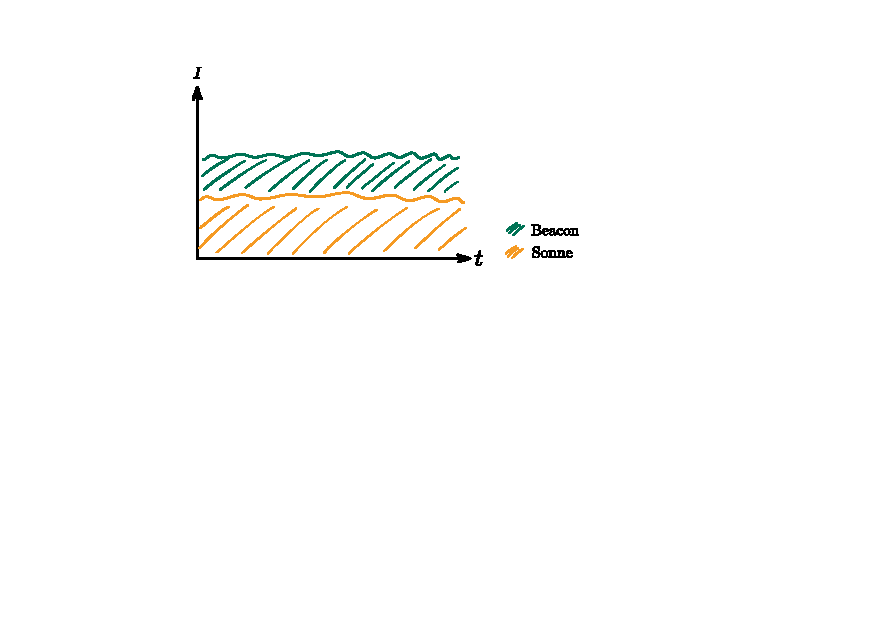
\includegraphics[width=\textwidth]{../assets/on-off-keying-1.pdf}
        \caption{Signalstärken ohne On"=Off"=Keying}
    \end{subfigure}
    \hspace{0.5cm}
    \begin{subfigure}{0.8\textwidth}
        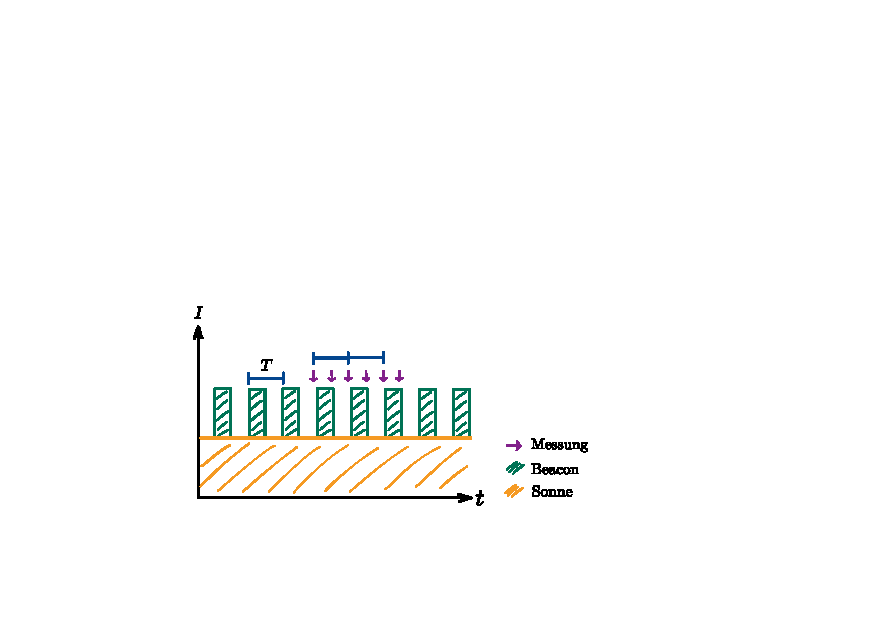
\includegraphics[width=\textwidth]{../assets/on-off-keying-2.pdf}
        \caption{Signalstärken mit On"=Off"=Keying (grün)}
    \end{subfigure}
    \caption{Diagramme der Signalstärke von Infrarot"=Signalen $I$ über die Zeit $t$ mit und ohne On"=Off"=Keying"=Prinzip zur Unterscheidung von Beacon und Sonne als exemplarische Störquelle (stark vereinfacht und nicht proportional)}
    \label{fig:on-off-keying}
\end{figure}

Da der Dezibot über keinen (Hardware"=) Bandpassfilter verfügt und die Berechnung in Software zu ressourcenintensiv wäre, muss ein optimierter Algorithmus entworfen werden. Dieser muss eine effiziente Filterung ermöglichen, um die Signale in Echtzeit zu unterscheiden.

Weiterhin wäre es möglich, dieses Problem zu lösen, in dem keine Infrarot"= sondern anderweitige, nicht natürlich vorkommende Signale verwendet werden, wie beispielsweise WLAN oder Bluetooth.

Mit dem Bluetooth 5.1 Standard wurde die \emph{Angle of Arrival} (AOA) Methode hinzugefügt. Damit ist es möglich, den Winkel bzw. die Richtung eines empfangenen Bluetooth"=Paketes zu approximieren~\cite[][Abschnitt 8.1]{bluetoothsigincBluetoothCoreSpecification2019}. Dies wäre sehr gut geeignet, um den Winkel des Beacons zu bestimmen, anstelle vom in \autoref{sec:angle-determination} erläuterten Algorithmus. Im Dezibot ist der ESP32-S3-MINI-1 verbaut~\cite{fingerleDokumentationDezibot42025}, welcher diese Methode jedoch (noch) nicht unterstützt~\cite{espressifsystemsshanghaico.ltdMajorFeatureSupport2024}.

Ein weiteres Problem besteht darin, dass sich der Dezibot bei der Rotation vom ursprünglichen Platz wegbewegt, da dieser sich nicht still um die eigene Achse drehen kann. Somit verändert sich der Beacon"=Winkel, selbst wenn der Dezibot sich nicht rotiert hat. Dieses Problem ist in \autoref{fig:dezibot_signal_moving_problem} veranschaulicht.

\begin{figure}[h]
    \centering
    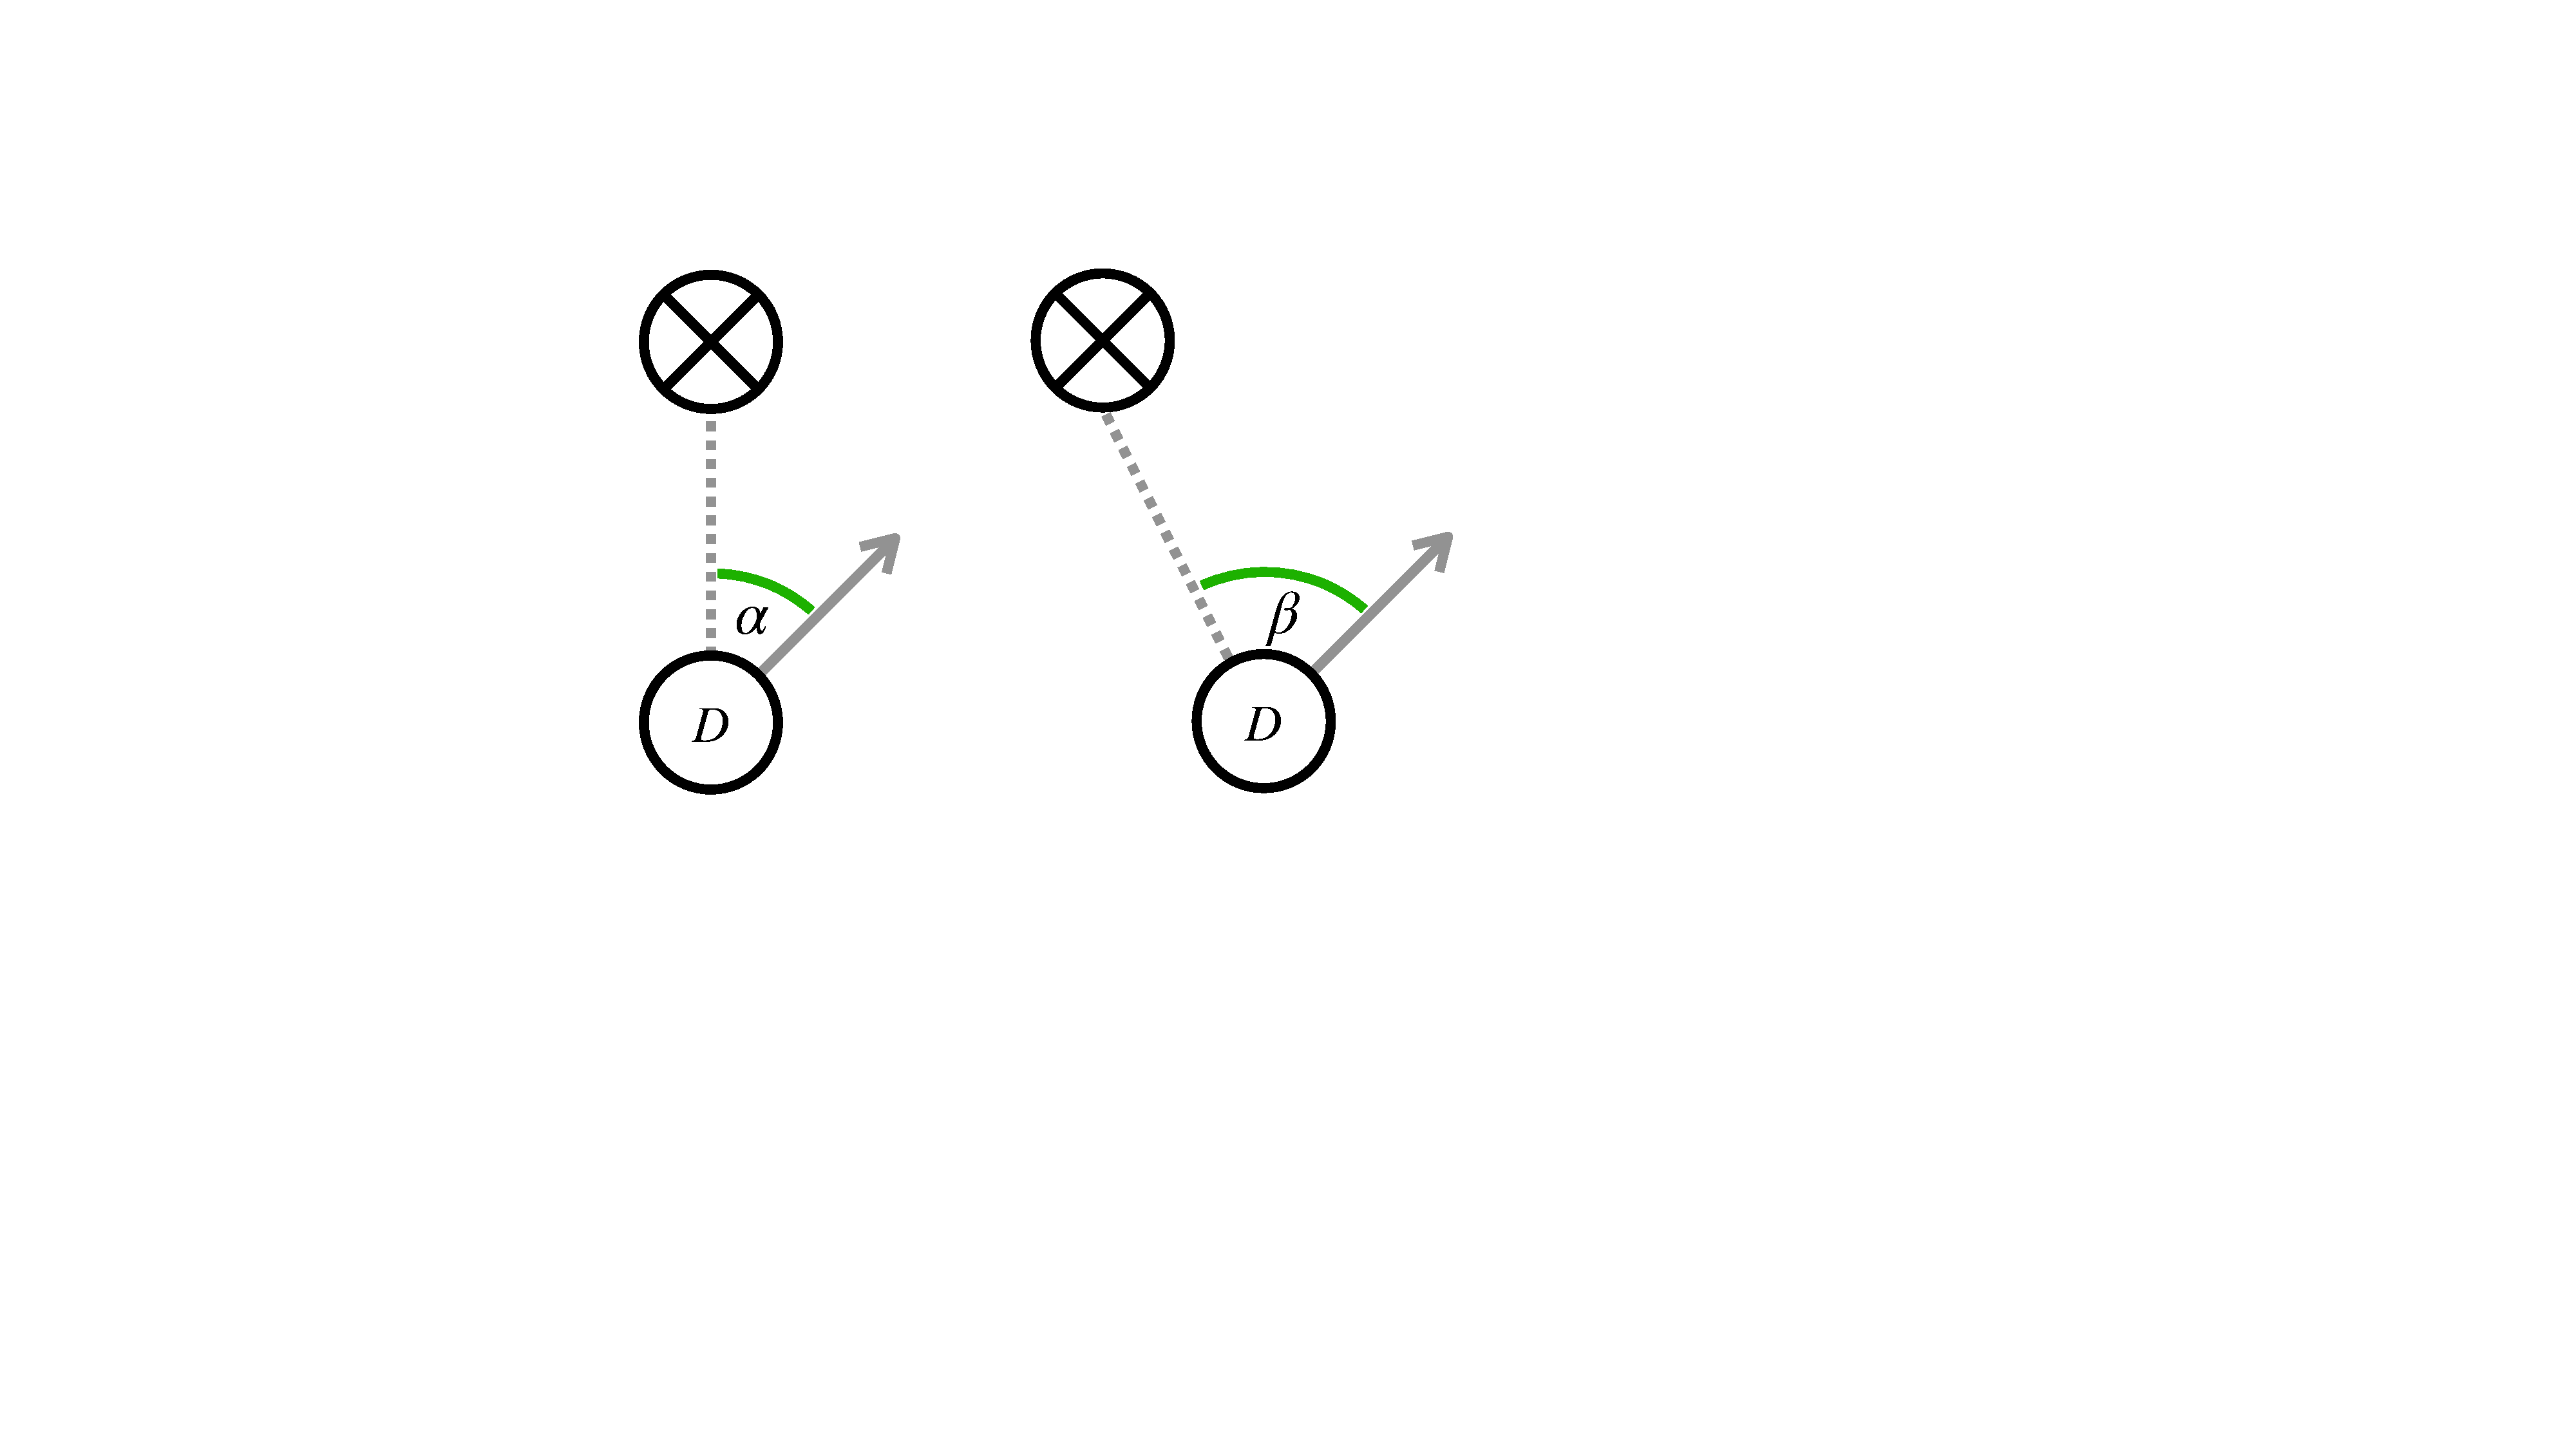
\includegraphics[width=0.5\textwidth]{../assets/dezibot_signal_moving_problem.pdf}
    \caption{Verändernder Beacon"=Winkel $\alpha$ bzw. $\beta$ bei Bewegung des Dezibots ohne Rotation.}
    \label{fig:dezibot_signal_moving_problem}
\end{figure}

Dabei ist dargestellt, wie sich der Beacon"=Winkel $\alpha$ zu $\beta$ verändert, wenn dieser die Position ändert, allerdings sich nicht rotiert, d.h. immer noch in die gleiche Richtung ausgerichtet ist. Dieser Fehler ist nicht trivial lösbar. Hierfür wäre eine Art Selbstortung des Dezibots notwendig, beispielsweise durch eine Triangulation mit einem zweiten Beacon. Dabei müssten die beiden Beacon unterschiedliche Frequenzen aussenden, damit sie unterscheidbar sind (vgl. erwähnter Ansatz oben).

Eine Selbstortung wäre durch mindestens drei weitere Beacon"=Dezibots denkbar, welche jeweils ein WLAN"=Signal aussenden. Durch die Messung der jeweiligen \emph{Wi-Fi Round Trip Time} (Wi-Fi RTT) wäre eine Triangulation der Position auf dem Schachbrett möglich. Ein ähnlicher Implementierungsansatz ist beispielhaft unter~\cite{espressifsystemsshanghaico.ltdFTMExample2024} einsehbar. Diese Methode setzt jedoch eine sehr genaue Zeitmessung voraus, welche mit dem Dezibot nicht unbedingt gegeben ist. Folglich stellt sich die Frage, ob diese Methode die notwendige Präzision erreichen kann.

% Zusammenfassung

Zusammenfassend unterscheiden sich die genannten Ansätze in ihrer Komplexität. In der begrenzten Projektzeit war es nicht möglich, diese weiter zu verfolgen, weshalb sie Forschungsgegenstand zukünftiger Projekte darstellen könnten.
